\documentclass{standalone}
\usepackage{tikz}
\usepackage{amsmath}
\usepackage{amssymb}

\begin{document}

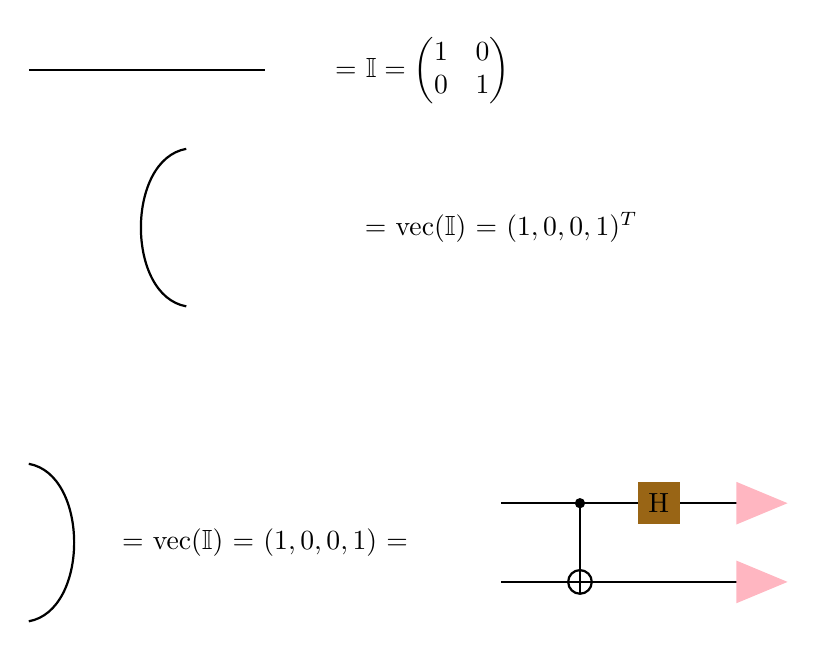
\begin{tikzpicture}

    \definecolor{pastelbrown}{RGB}{153,101,21}
    \definecolor{pastelred}{RGB}{255,182,193}
    % Draw the line and label it as equivalent to the identity matrix
    \draw[thick] (1,0) -- (4,0);
    
    % Draw the identity matrix
    \node at (6,0) {= $\mathbb{I} = \begin{pmatrix}
        1 & 0 \\
        0 & 1
    \end{pmatrix}$};
    
    % Draw the curved line and label it as equivalent to the vector (1,0,0,1)
    \draw[thick] (3,-1) to[out=-170,in=170] (3,-3);
    
    % Draw the vector
    \node at (7,-2) {= vec($\mathbb{I}$) = $(1,0,0,1)^T$};

    % Draw the curved line and label it as equivalent to the vector (1,0,0,1)
    \draw[thick] (1,-5) to[out=-10,in=10] (1,-7);
    
    % Draw the vector
    \node at (4,-6) {= vec($\mathbb{I}$) = $(1,0,0,1)$ = };

    \draw[thick] (7,-5.5) to (10,-5.5);
    \draw[thick] (7,-6.5) to (10,-6.5);
    \draw[thick] (8,-5.5) to (8,-6.65);
    \filldraw[pastelbrown, thick] (8.75,-5.75) rectangle (9.25,-5.25);
    \filldraw[pastelred, thick] (10.6,-5.5) -- (10,-5.25) -- (10,-5.75) -- cycle;
    \filldraw[pastelred, thick] (10.6,-6.5) -- (10,-6.25) -- (10,-6.75) -- cycle;
    \filldraw[black, thick] (8,-5.5) circle (0.05); 
    \draw[thick] (8,-6.5) circle(0.15);
    \node at (9,-5.5) {H};
    

    
    

\end{tikzpicture}

\end{document}
